% include the figures path relative to the master file
% \graphicspath{ {./content/method/figures/visual_cues/}{./content/method/figures/}}
\graphicspath{ {./content/method/figures/}}

\section{Materials and Methods}\label{sec:method}

The proposed method, as well as, its experimental set-up for \ac{oct} volume classification are outlined in Fig.\,\ref{fig:ML-scheme}.
The methodology is formulated as a standard classification procedure which consists of five steps.
First, the \ac{oct} volumes are pre-processed as presented in details in Sect.\,\ref{subsec:prepro}.
Then, \ac{lbp} and \ac{lbptop} features are detected, mapped and represented as discussed in depth in Sect.\,\ref{subsec:feaext}, Sect.\,\ref{subsec:mapping}, and Sect.\,\ref{subsec:fearep}, respectively.
Finally, the classification step is presented in Sect.\,\ref{subsec:cls}.


\subsection{Image pre-processing}\label{subsec:prepro}

This section describes the set of pre-processing techniques which aim at enhancing the \ac{oct} volume.
The influence of these pre-processing methods and their possible combinations are extensively studied in Sect.\,\ref{sec:exp}.

\subsubsection{\acf{nlm}}

\begin{figure}[t]
  \centering
  \hspace*{\fill}
  \subfigure[]{\label{subfig:vol}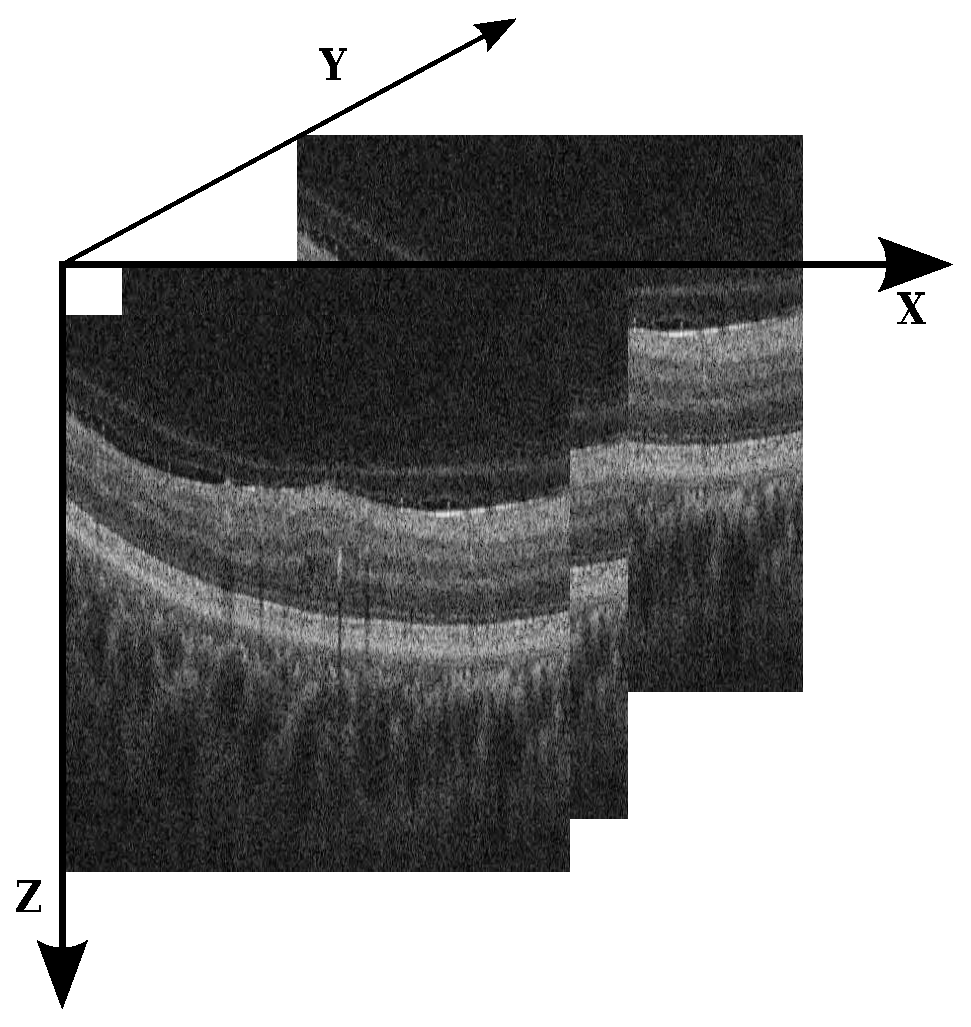
\includegraphics[width=0.3\linewidth]{axs}} \hfill
  \subfigure[]{\label{subfig:raw}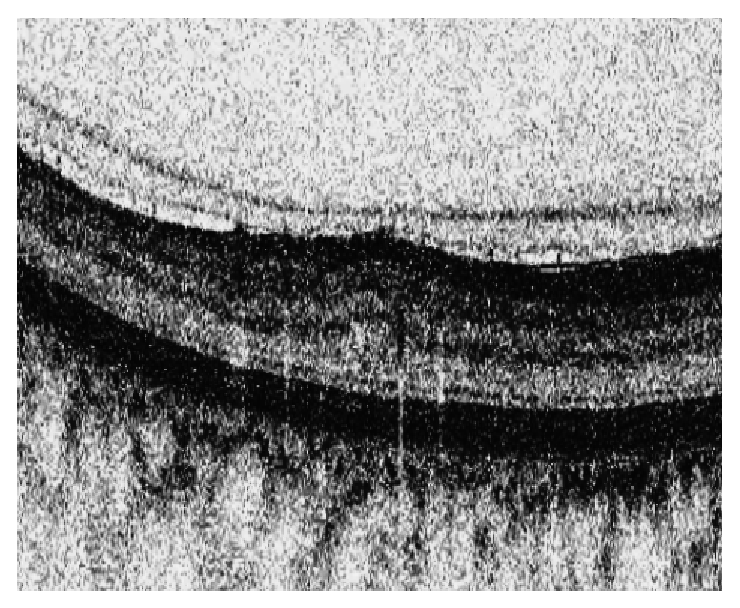
\includegraphics[width=0.3\linewidth]{raw_crop_grey}} \hfill
  \subfigure[]{\label{subfig:nlm}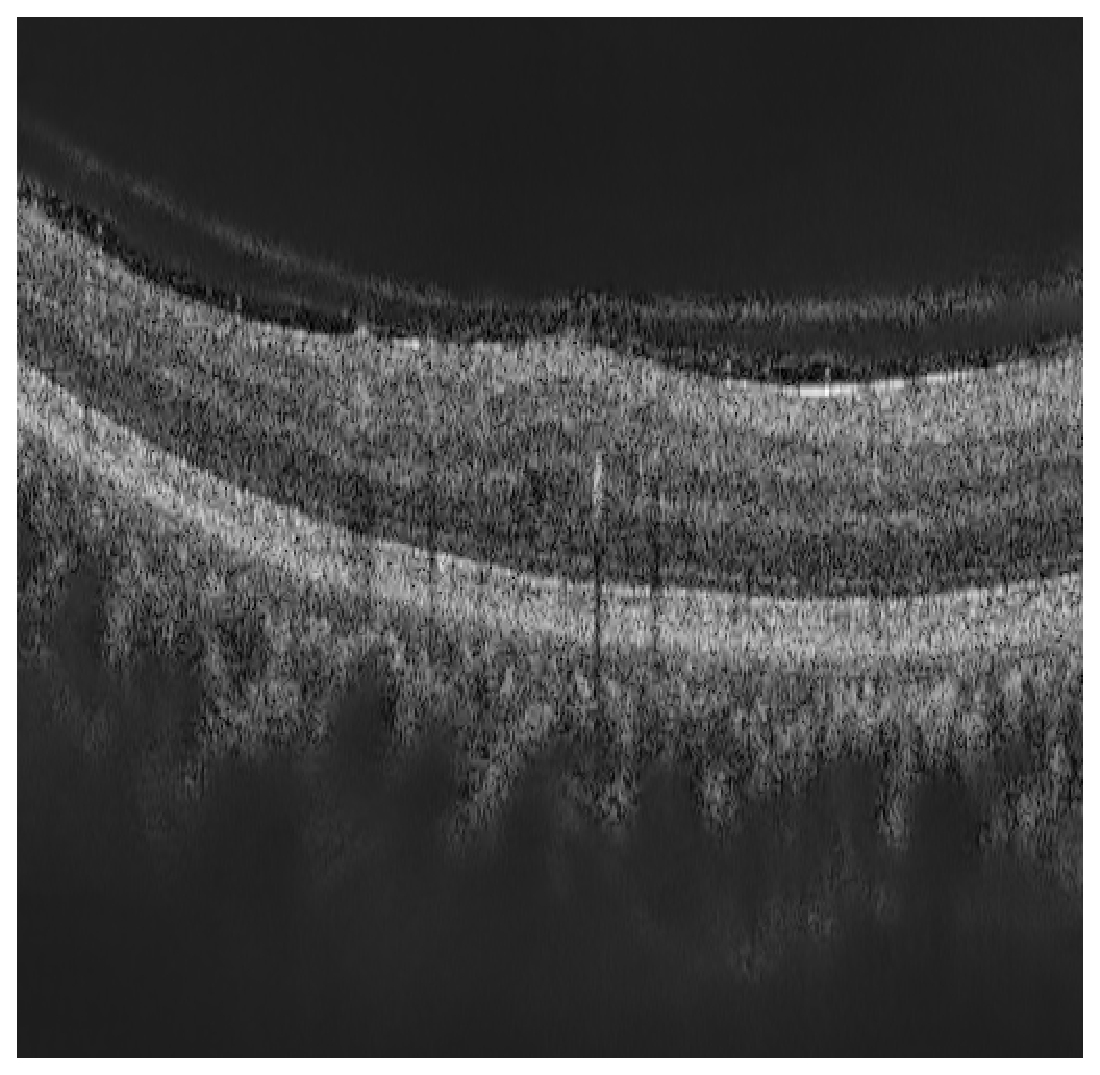
\includegraphics[width=0.3\linewidth]{nlm_crop_grey}}
  \hspace*{\fill}
  \caption{\ac{oct}: (a) Organization of the \ac{oct} data - (b) Original image - (c) \ac{nlm} filtering. Note that the images have been negated for visualization purposes.}
  \label{fig:denoise}
\end{figure}


\ac{oct} images suffer from speckle noise, like other image modalities such as \ac{us}~\cite{schmitt1999speckle}.
The \ac{oct} volumes are enhanced by denoising each B-scan (i.e. each $(x$-$z)$ slice) using the \ac{nlm}~\cite{buades2005non}, as shown in Fig.\,\ref{fig:denoise}.
\ac{nlm} has been successfully applied to \ac{us} images to reduce speckle noise and outperforms other common denoising methods~\cite{Coupe2009}.
\ac{nlm} filtering preserves fine structures as well as flat zones, by using all the possible self-predictions that the image can provide rather than local or frequency filters such as Gaussian, anisotropic, or Wiener filters~\cite{buades2005non}.

\subsubsection{Flattening}

\begin{figure}[t]
\centering 
  \hspace*{\fill}
  \subfigure[]{\label{subfig:flatorg}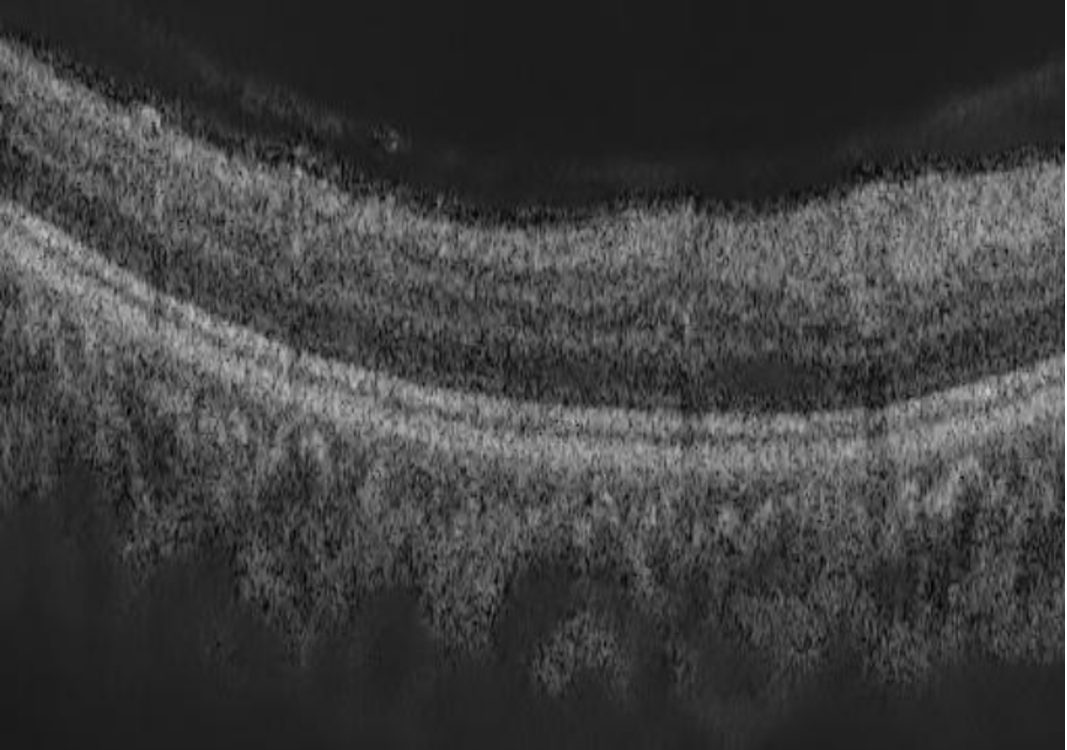
\includegraphics[width=0.20\textwidth]{flattening/original_cropped}}\hfill
  \subfigure[]{\label{subfig:flatotsu}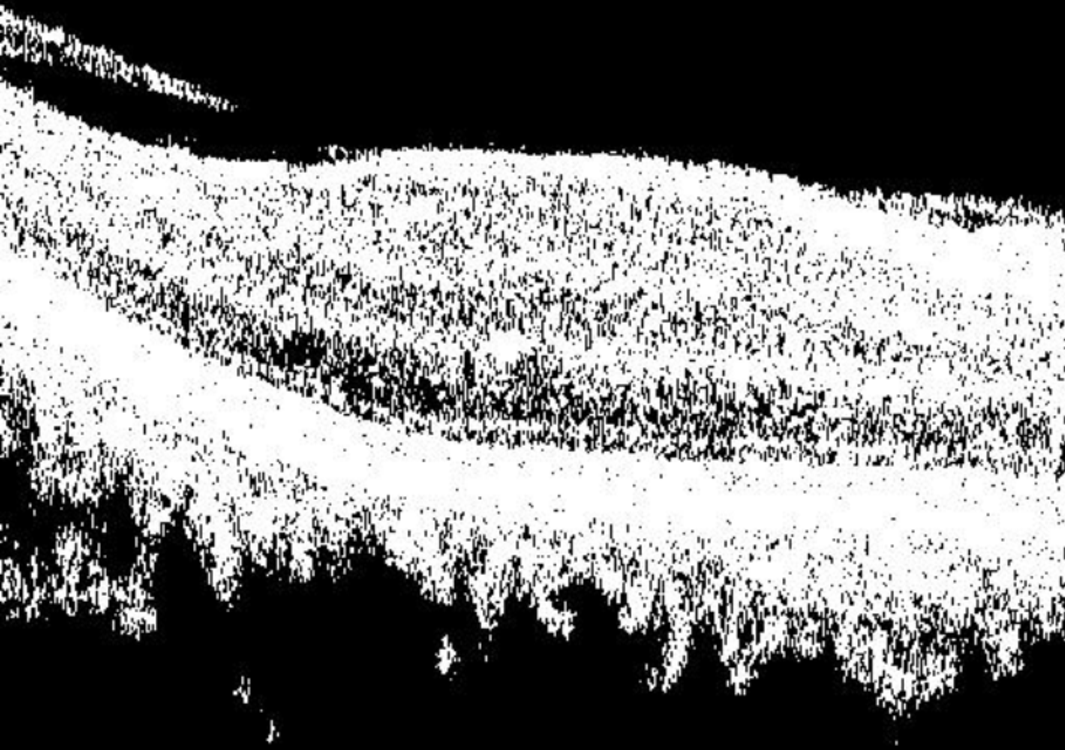
\includegraphics[width=0.20\textwidth]{flattening/thresholding_cropped}}\hfill
  \subfigure[]{\label{subfig:flatmedian}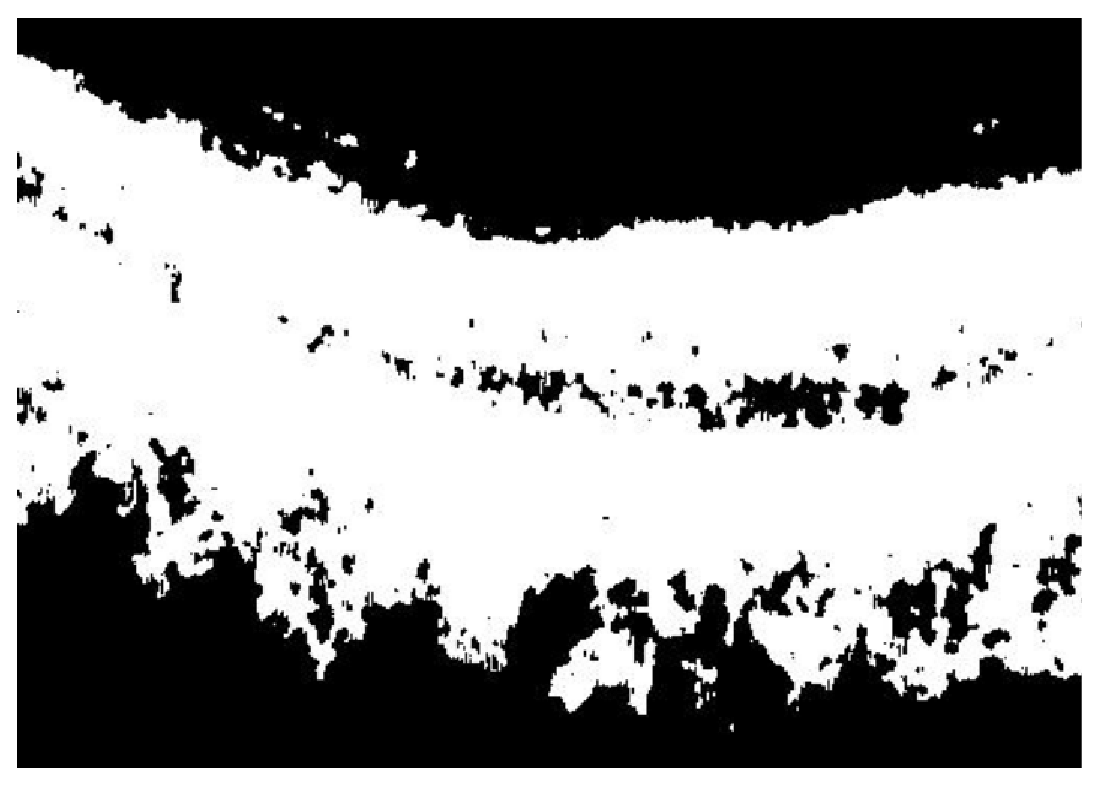
\includegraphics[width=0.20\textwidth]{flattening/median_cropped}}
  \hspace*{\fill}	
  \\
  \hspace*{\fill}
  \subfigure[]{\label{subfig:flatfit}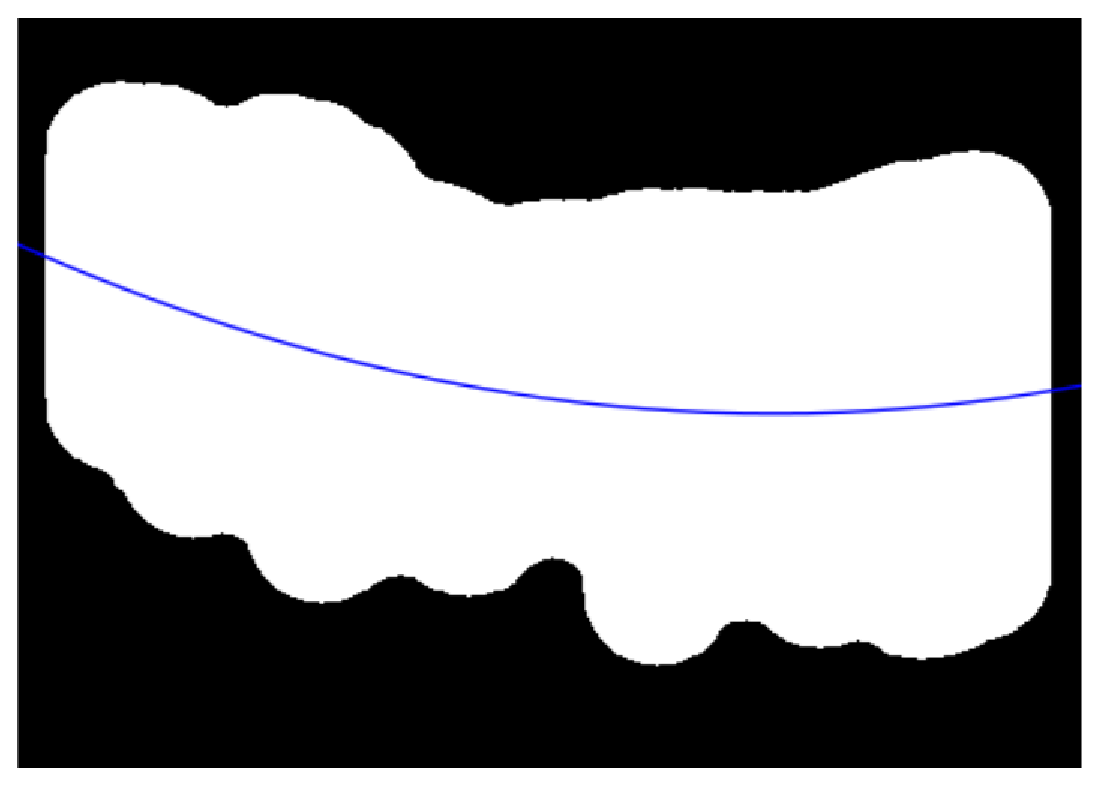
\includegraphics[width=0.20\textwidth]{flattening/fit_cropped}}\hfill
  \subfigure[]{\label{subfig:flatwarp}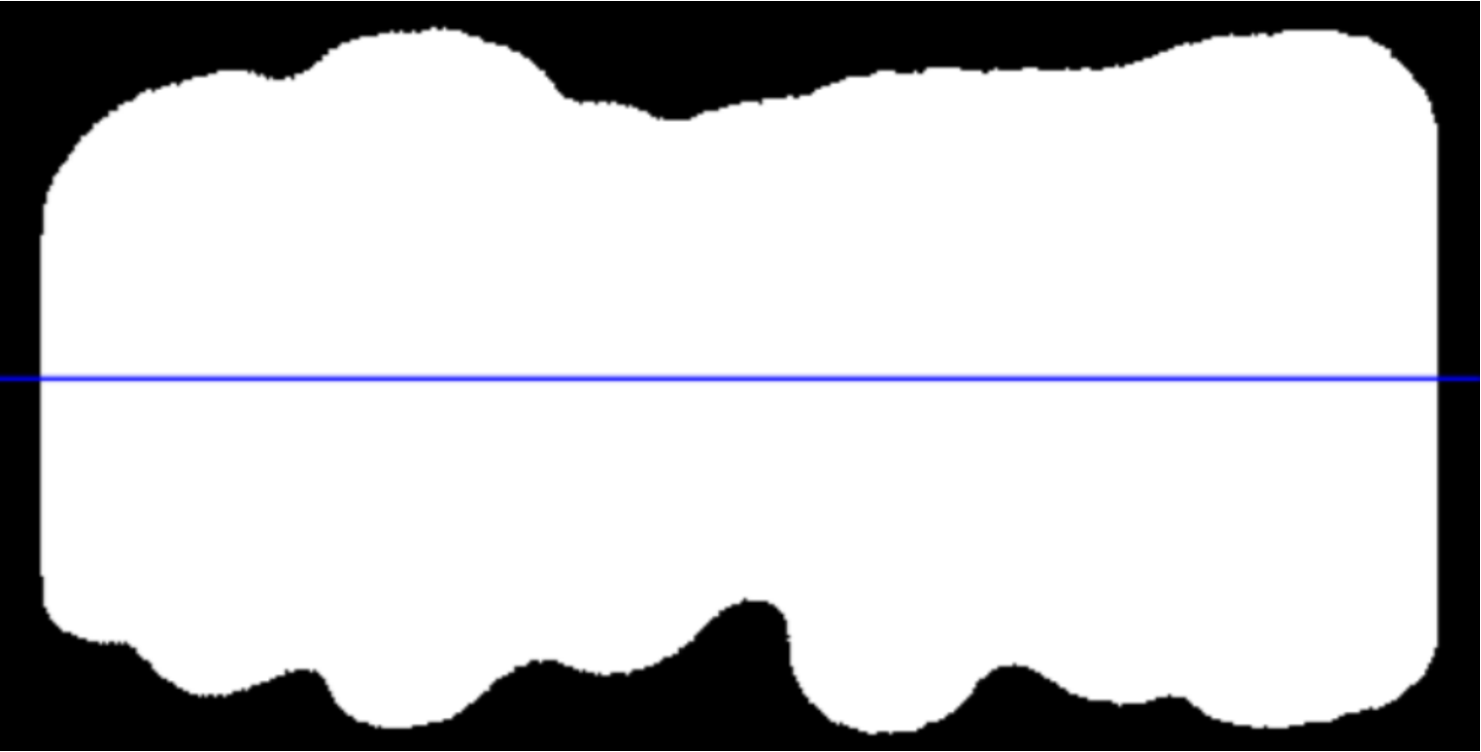
\includegraphics[width=0.20\textwidth]{flattening/warped_cropped}}\hfill
  \subfigure[]{\label{subfig:flatfinal}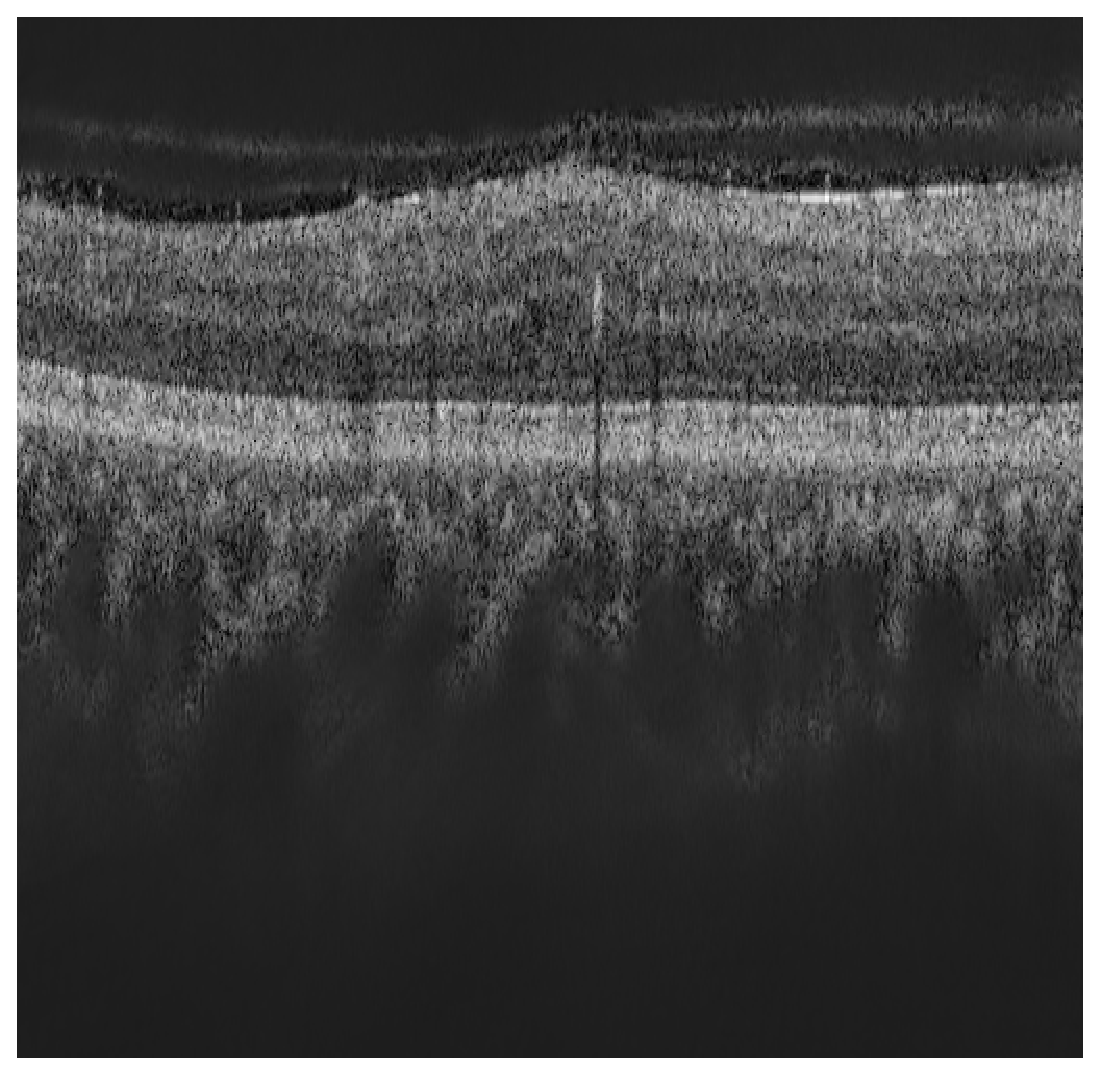
\includegraphics[width=0.20\textwidth]{flattening/warped_org_cropped}}
  \hspace*{\fill}
  \caption{Flattening procedure: (a) original image, (b) thresholding, (c) median filtering, (d) curve fitting, (e) warping, (f) flatten image.}
  \label{fig:flatten}
\end{figure}

Textural descriptors characterize spatial arrangement of intensities.
However, the \ac{oct} scans suffer from large type of variations: inclination angles, positioning, and natural curvature of the retina~\cite{Liu2011}.
Therefore, these variations have to be taken into account to ensure a consistent characterization of the tissue disposition, regardless of the location in the retina.
This invariance can be achieved from different manners: (i) using a rotation invariant descriptor (cf. Sect.\,\ref{subsec:feaext}), or (ii) by unfolding the curvature of the retina.
This latter correction is known as image flattening which theoretically consists of two distinct steps: (i) estimate and fit the curvature of the \ac{rpe} and (ii) warp the \ac{oct} volume such that the \ac{rpe} becomes flat.

Our correction is similar to the one of Liu\,\textit{et~al.}~\cite{Liu2011}: each B-scan is thresholded using Otsu's method followed by a median filtering to detect the different retina layers (see Fig\,\ref{subfig:flatmedian} and Fig\,\ref{subfig:flatotsu}). 
Then, a morphological closing and opening is applied to fill the holes and the resulting area is fitted using a second-order polynomial (see Fig.\,\ref{subfig:flatfit}). 
Finally, the scan is warped such that the curve becomes a line as presented in Fig.\,\ref{subfig:flatwarp} and Fig.\,\ref{subfig:flatfinal}. 

\subsubsection{Slice alignment}
The flattening correction does not enforce an alignment through the \ac{oct} volume.
Thus, in addition to the flattening correction, the warped curves of each B-scan are positioned at the same altitude in the $z$ axis. 

\subsection{Feature detection}\label{subsec:feaext}
In this research, we choose to detect simple and efficient \ac{lbp} texture features with regards to each \ac{oct} slice and volume.
\ac{lbp} is a texture descriptor based on the signs of the differences of a central pixel with respect to its neighboring pixels~\cite{ojala2002multiresolution}.
These differences are encoded in terms of binary patterns as in~Eq.\,\eqref{Eq:LBP}:

\begin{equation}\label{Eq:LBP}
LBP_{P,R} = \sum_{p=0}^{P-1}s(g_{p} - g_{c})2^{p} \ , \qquad s(x) = \begin{cases}
    1  & \ \text{if } x \geq 0\\
    0  & \ \text{otherwise}\\
  \end{cases} \ ,
\end{equation}

\noindent where $g_c$, $g_{p}$ are the intensities of the central pixel and a given neighbor pixel, respectively; $P$ is the number of sampling points in the circle of radius $R$.

Ojala\,\textit{et~al.} further extended the original \ac{lbp} formulation to achieve rotation invariance at the expense of limiting the texture description to the notion of circular ``uniformity''~\cite{ojala2002multiresolution}.
Referring to the coordinate system defined in Fig.\,\ref{subfig:vol}, the \ac{lbp} codes are computed on each $(x$-$z)$ slice, leading to a set of \ac{lbp} maps, a map for each $(x$-$z)$ slice.

Volume encoding is later proposed by Zhao\,\textit{et~al.} by computing \ac{lbp} descriptors in three orthogonal planes, so called \ac{lbptop}~\cite{zhao2012rotation}.
More precisely, the \ac{lbp} codes are computed considering the $(x$-$z)$ plane, $(x$-$y)$ plane, and $(y$-$z)$ plane, independently.
Thus, three sets of \ac{lbp} maps are obtained, one for each orthogonal plane.

In this work, we consider rotation invariant and uniform \ac{lbp} and \ac{lbptop} features with various sampling points (i.e., $\{8,16,24\}$) with respect to different radius, (i.e., $\{1,2,3\}$).
The number of patterns ($LBP_{\#pat}$) in regards with each configuration is reported in Table~\ref{tab:lbphist}.

\begin{table}
\caption{Number of patterns ($LBP_{\#pat}$) for different sampling points and radius ($\{P,R\}$) of the \ac{lbp} descriptor.}
\centering{
\resizebox{0.5\linewidth}{!}{
\footnotesize{
\begin{tabular}{l  c c c }
\toprule
 \multicolumn{4}{c}{Sampling point for a radius ($\{P, R\}$)}\\
 \midrule
 & $\{8, 1\}$ & $\{16, 2\}$ & $\{24, 3\}$\\
 \cmidrule{2-4}
  $LBP_{\#pat}$  & 10 & 18 & 26 \\
 \bottomrule
\end{tabular}}}}
\label{tab:lbphist}
\end{table}

\subsection{Mapping} \label{subsec:mapping}
The mapping stage is used to partition the previously computed \ac{lbp} maps; for this work, two mapping strategies are defined: (i) \emph{global} and (ii) \emph{local} mapping.
The size of the feature descriptor is summarized in Table~\ref{tab:descsize}.

\begin{table}
\caption{Size of a descriptor for an \ac{sdoct} volume. $d$ denotes the number of slices in the volume, $N$ the number of 2D windows, and $N'$ the number of 3D sub-volumes, respectively.}
\centering{
\footnotesize{
\begin{tabular}{l c c }
  \ctoprule{2-3}
  & Global mapping & Local mapping \\
  \midrule
  \ac{lbp} & $d \times LBP_{\#pat}$ & $(N \times d) \times LBP_{\#pat}$ \\
  \midrule
  \ac{lbptop} & $1 \times (3 \times LBP_{\#pat})$ & $N' \times (3 \times LBP_{\#pat})$ \\
  \bottomrule
\end{tabular}}}
\label{tab:descsize}
\end{table}

\begin{figure}[t]
  \centering
  \hspace*{\fill}
  \subfigure[]{\label{subfig:glbp}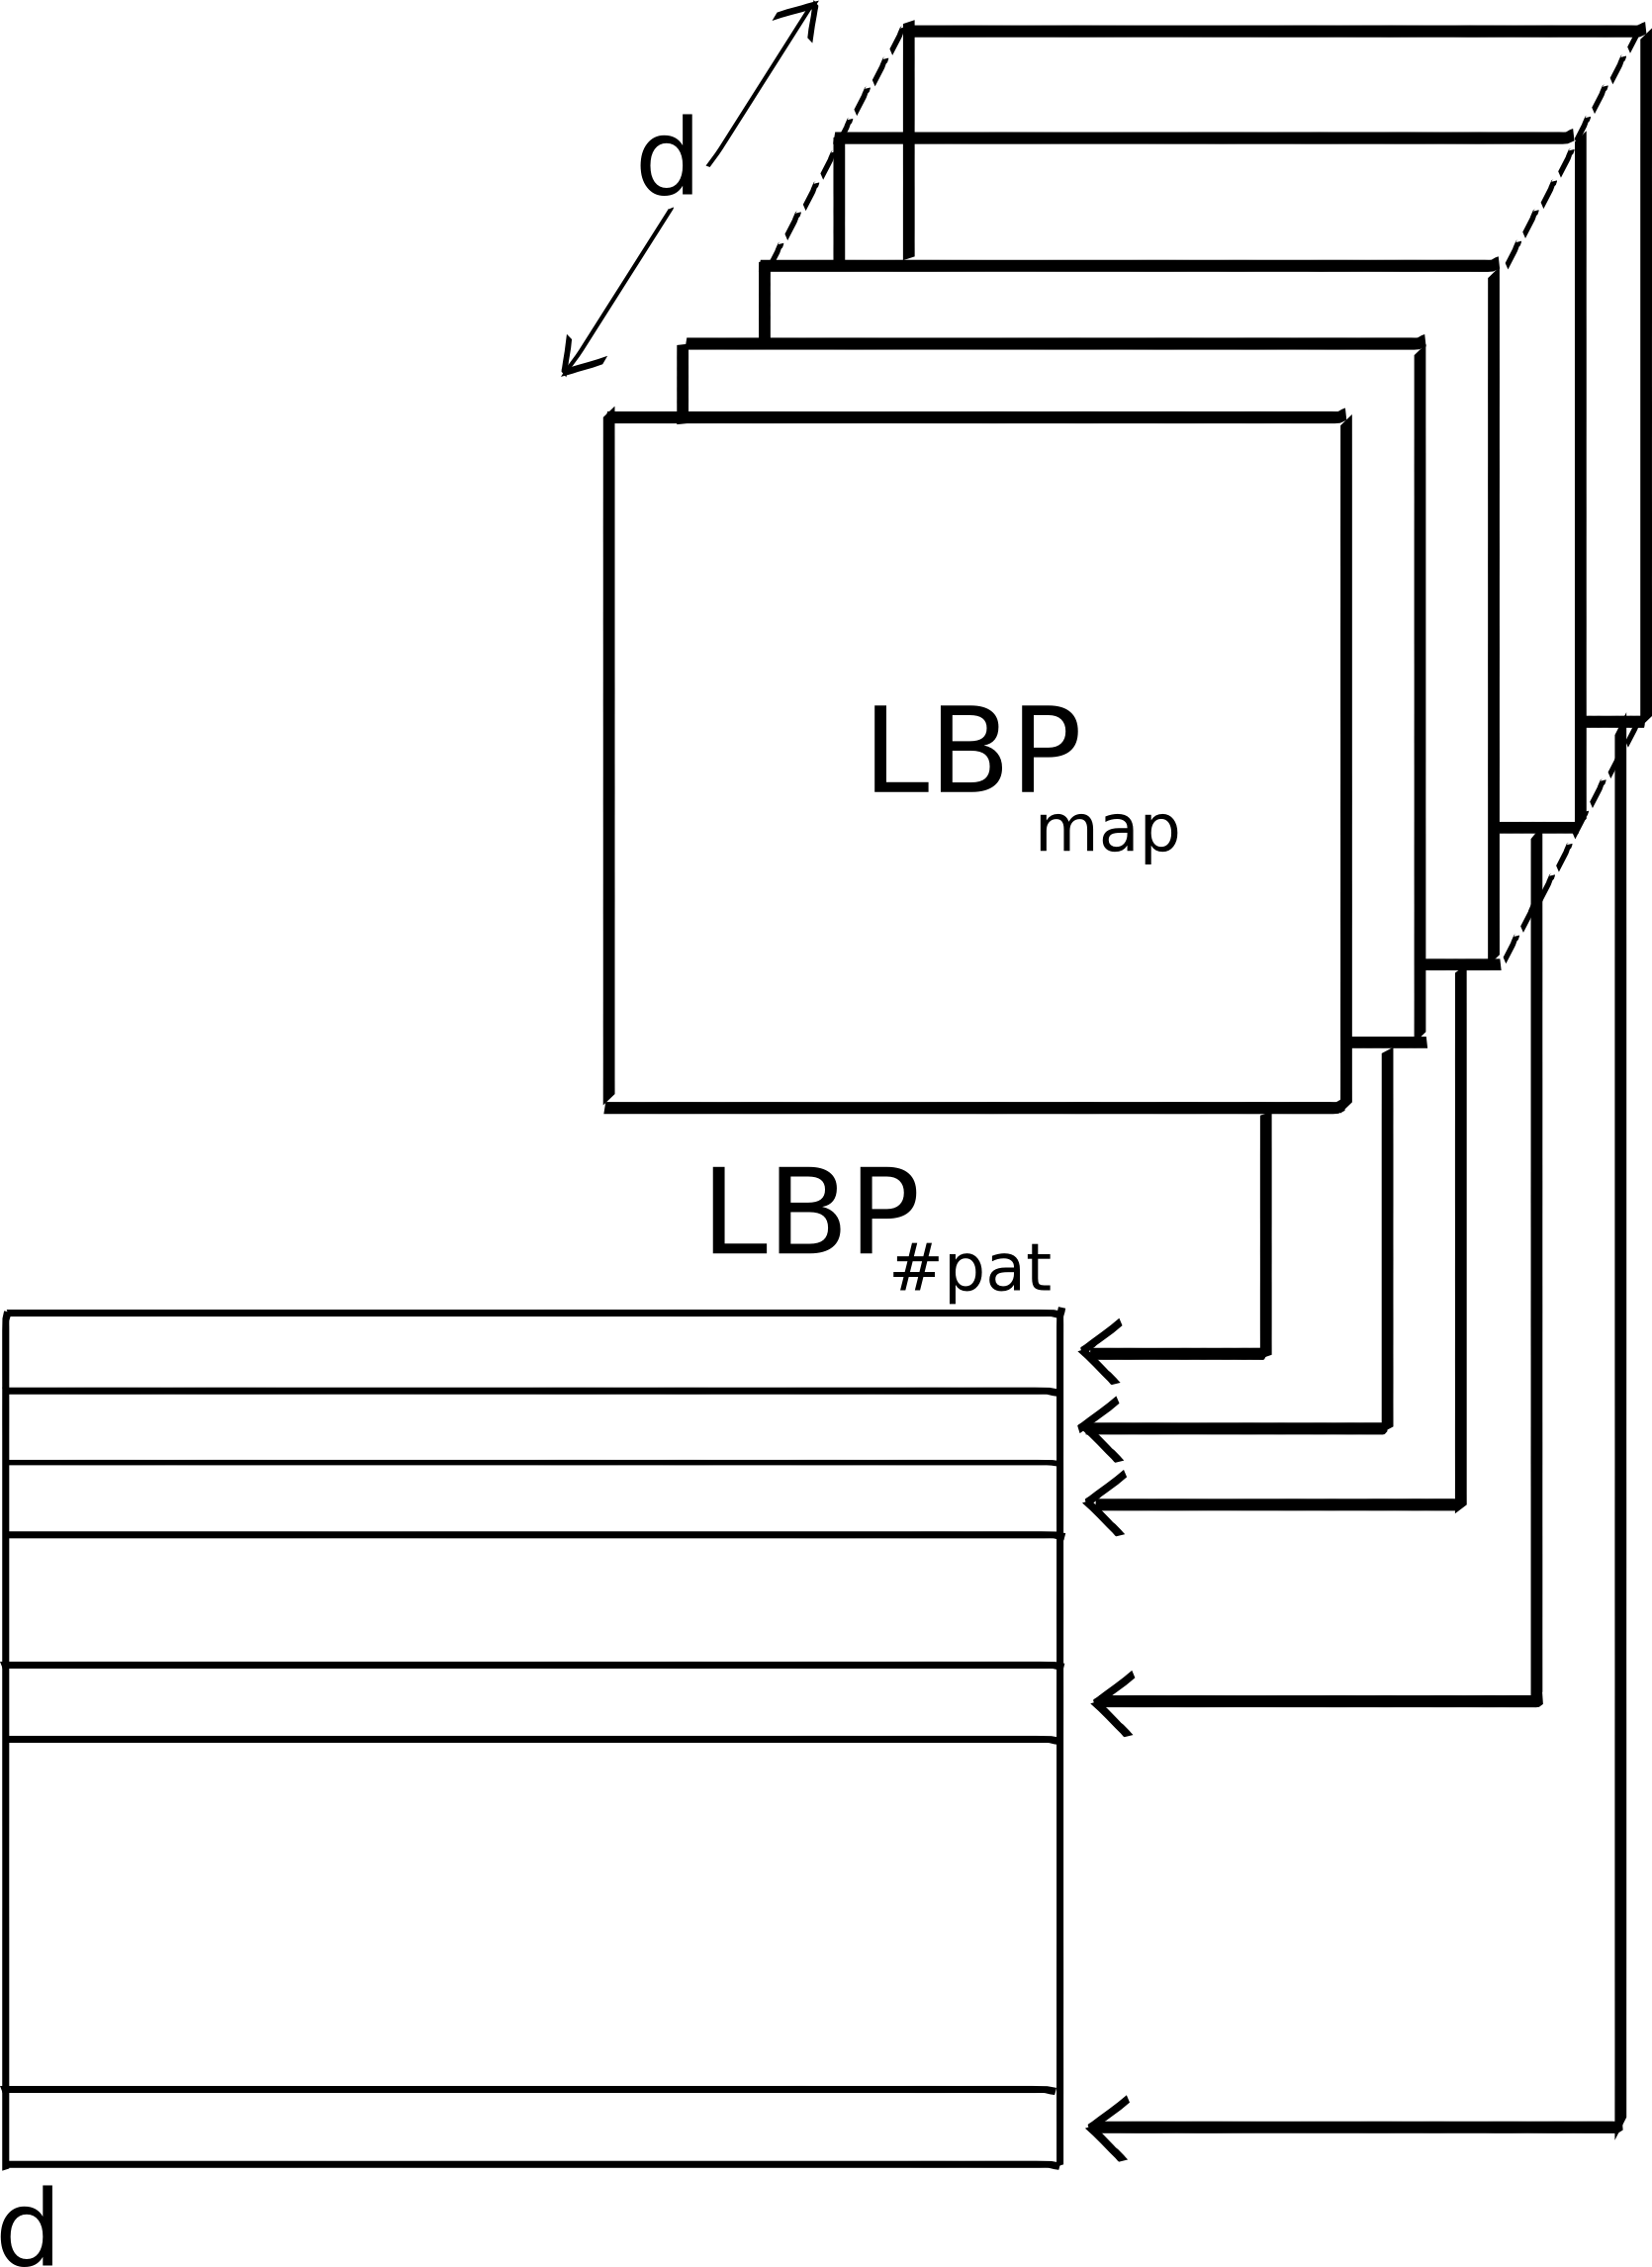
\includegraphics[width=0.25\linewidth]{global-lbp}} \hfill
  \subfigure[]{\label{subfig:glbptop}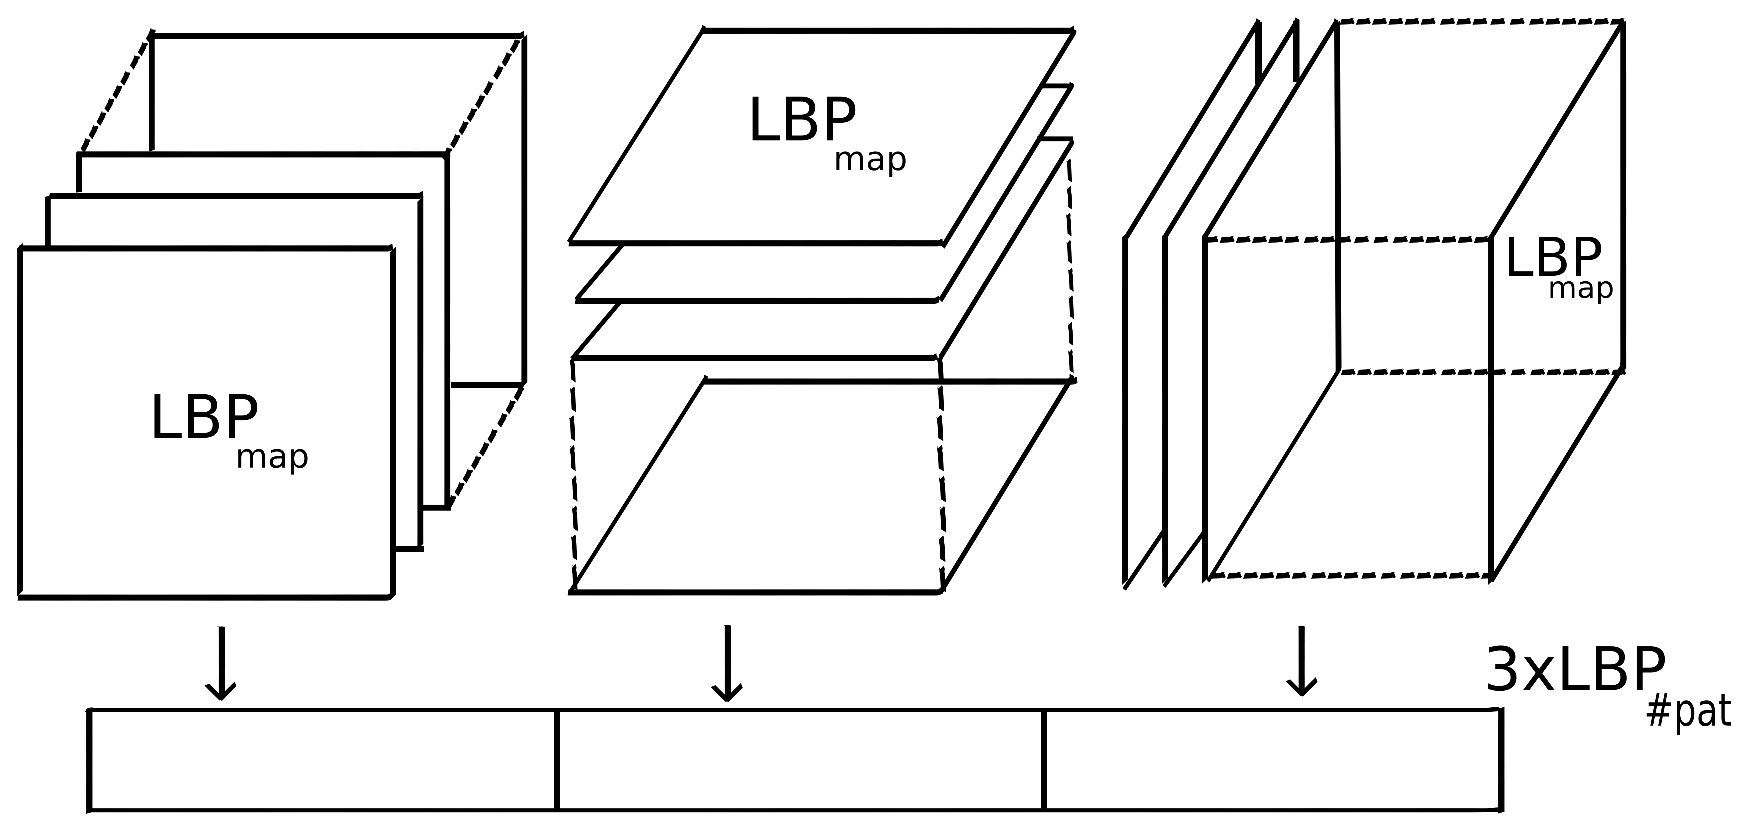
\includegraphics[width=0.48\linewidth]{global-lbptop}}
  \hspace*{\fill}\\
  \hspace*{\fill}
  \subfigure[]{\label{subfig:llbp}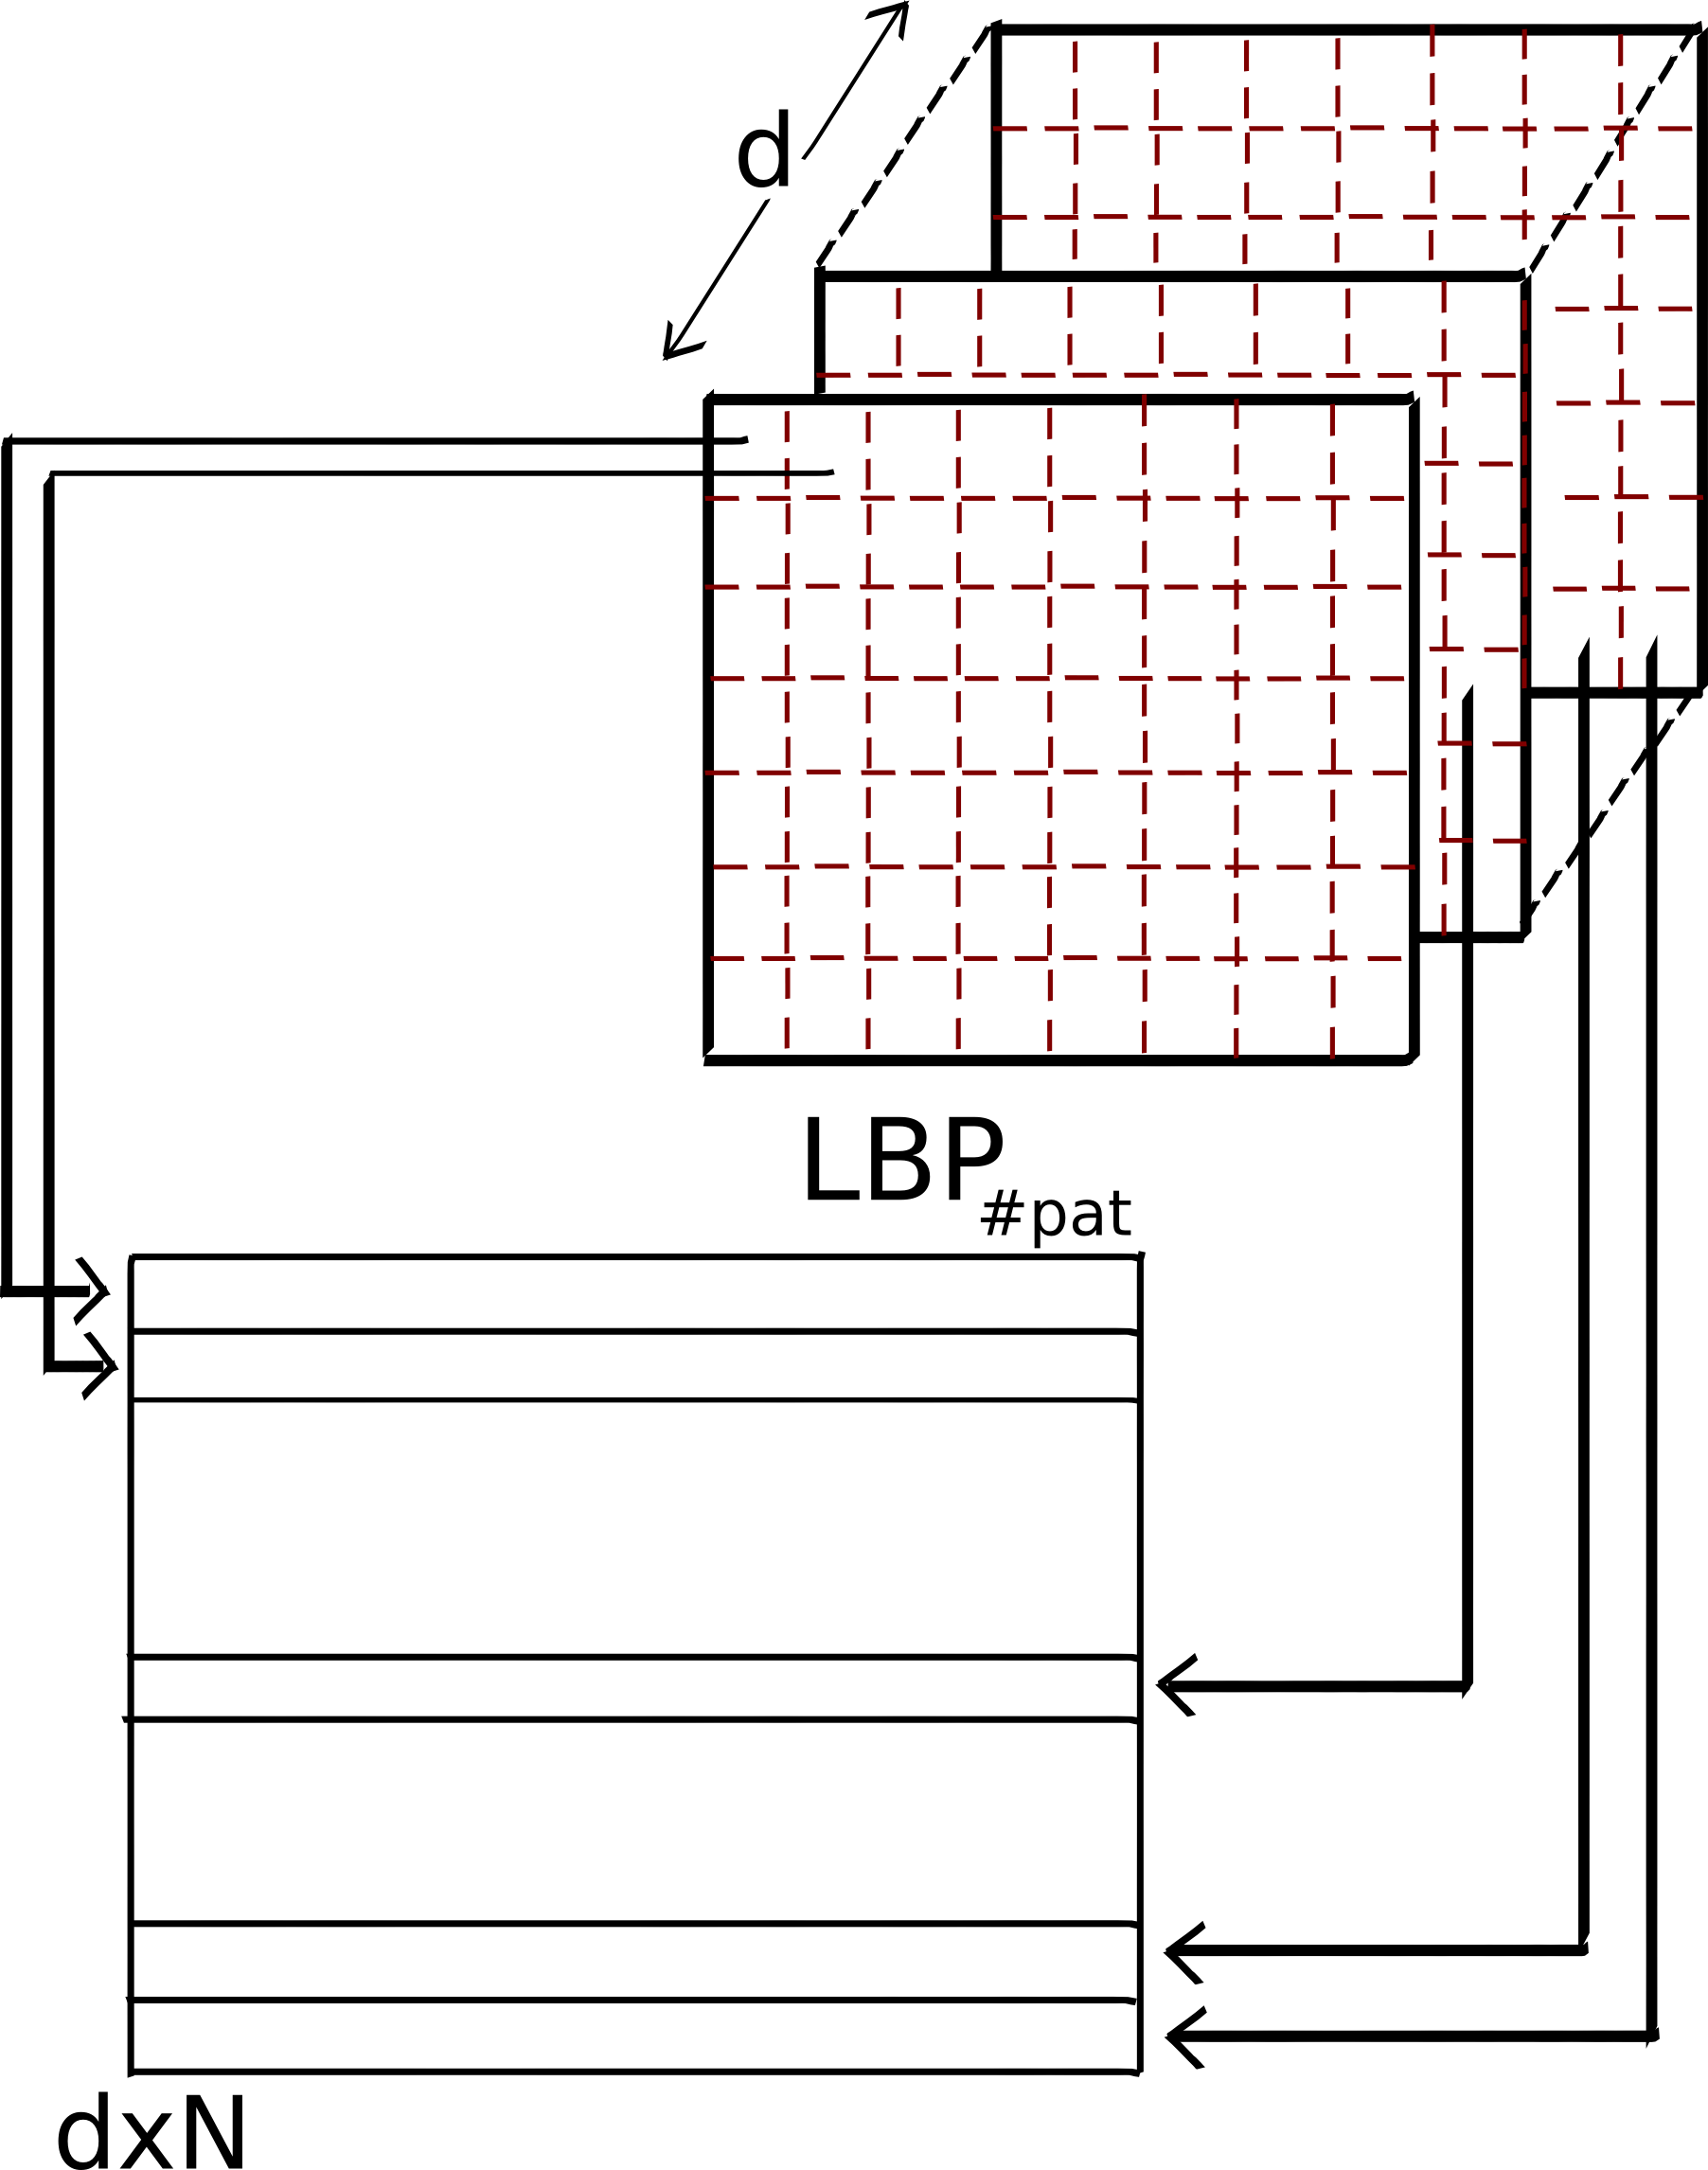
\includegraphics[width=0.25\linewidth]{local-lbp}} \hfill
  \subfigure[]{\label{subfig:llbptop}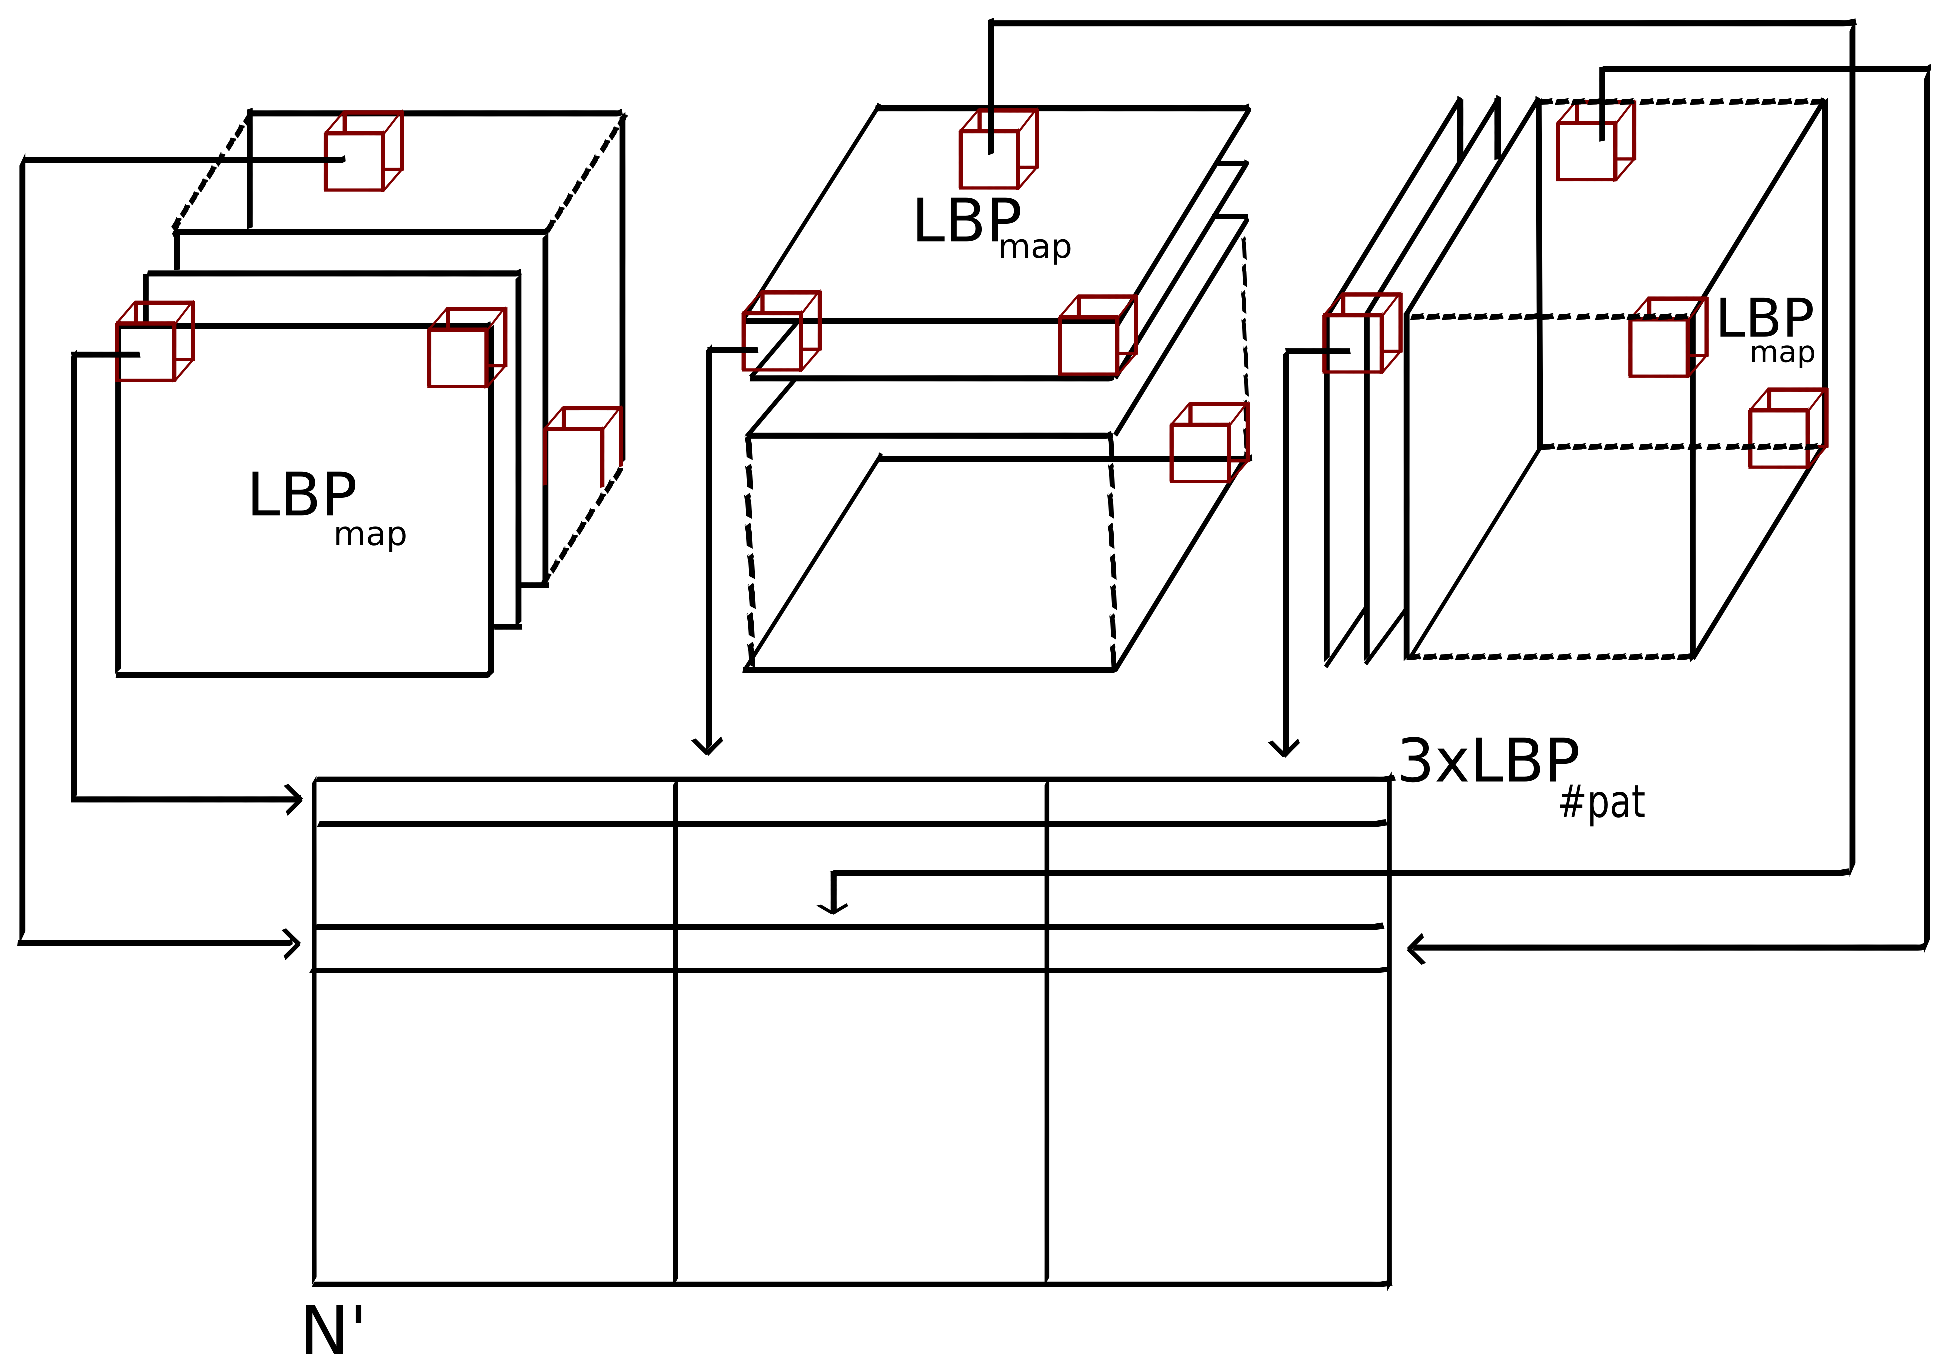
\includegraphics[width=0.48\linewidth]{local-lbptop}}
  \hspace*{\fill}
  \caption{Graphical representation of the feature extraction: (a) extraction of \ac{lbp} for global mapping - (b) extraction of \ac{lbptop} for global mapping - (c) extraction of \ac{lbp} for local mapping - (d) extraction of \ac{lbptop} for local mapping.}
  \label{fig:feaextimg}
\end{figure}

\begin{description}
\item[\emph{Global}] mapping extracts the final descriptors from the 2D feature image for \ac{lbp} and 3D volume for \ac{lbptop}.
%mapping considers to extract the features from the 2D B-scans for \ac{lbp} and 3D volume for \ac{lbptop}.
Therefore, for a volume with $d$ slices, the \emph{global}-\ac{lbp} mapping will lead to the extraction of $d$ elements.
While the \emph{global}-\ac{lbptop} represents the whole volume as a single element.
The \emph{global} mapping for 2D images and 3D volume is shown in Fig.~\ref{subfig:glbp} and \ref{subfig:glbptop}.

\item[\emph{Local}] mapping extracts the final descriptors from a set of ($m \times m$) 2D patches for \ac{lbp} and a set of ($ m \times m \times m$) sub-volumes for \ac{lbptop}.
Given $N$ and $N'$ the total number of 2D patches and 3D sub-volumes respectively, the \emph{local}-\ac{lbp} approach provides $N \times d$ elements, while \emph{local}-\ac{lbptop} provides $N'$ elements.
%Here $N$ and $N'$ are the total number of elements per B-scane or the volume, respectively.
This mapping is illustrated in Fig.~\ref{subfig:llbp} and \ref{subfig:llbptop}.

\end{description}

\subsection{Feature representation}\label{subsec:fearep}

Two strategies are used to describe each \ac{oct} volume's texture.

\begin{description}

\item[Low-level representation] The texture descriptor of an \ac{oct} volume is defined as the concatenation of the \ac{lbp} histograms with the \emph{global}-mapping.
The \ac{lbp} histograms are extracted from the previously computed \ac{lbp} maps (see Sect.\,\ref{subsec:feaext}).
Therefore, the \ac{lbptop} final descriptor is computed through the concatenation of the \ac{lbp} histograms of the three orthogonal planes with the final size of $3 \times LBP_{\#pat}$.
More precisely, an \ac{lbp} histogram is computed for each set of \ac{lbp} maps $(x$-$z)$ plane, $(x$-$y)$ plane, and $(y$-$z)$ plane, respectively.
Similarly, the \ac{lbp} descriptor is defined through concatenation of the \ac{lbp} histograms per each $(x$-$z)$ slice with the final size of $d \times LBP_{\#pat}$.

\item[High-level representation] The concatenation of histograms employed in the low-level representation in conjunction with either \emph{global}- or \emph{local}-mapping can lead to a high dimensional feature space.
For instance, \emph{local}-mapping results in a size of $N \times d \times LBP_{\#pat}$ for the final \ac{lbp} descriptor and $N' \times LBP_{\#pat}$ for the final \ac{lbptop} descriptor, where $N$ and $N'$ are the total number of 2D patches and 3D sub-volumes, respectively.
High-level representation simplifies this high dimensional feature space into a more discriminant lower space.
\ac{bow} approach is used for this purpose~\cite{Sivic2003}.
This model represents the features by creating a codebook or visual dictionary, from the set of low-level features.
The set of low-level features are clustered using \textit{k}-means to create the codebook with \textit{k} clusters or visual words.
After creating the codebook from the training set, the low-level descriptors are replaced by their closest word within the codebook.
The final descriptor is a histogram of size \textit{k} which represents the codebook occurrences for a given mapping.

\end{description}

\subsection{Classification}\label{subsec:cls}

The last step of our framework consists in the classification of \ac{sdoct} volumes as normal or \ac{dme}.
For that matter, five different classifiers are used: (i) $k$-\acf{nn}, (ii) \acf{lr}~\cite{cox1958regression}, (iii) \acf{rf}~\cite{breiman2001random}, (iv) \acf{gb}~\cite{friedman2002stochastic, lemaitre2015boosting}, and (v) \acf{svm}~\cite{vapnik1963generalized, aizerman1964}.
Details regarding the parameters used in our experiments are provided in Sect.\,\ref{sec:exp}.

%%% Local Variables:
%%% mode: latex
%%% TeX-master: "../../main.tex"
%%% End:
